\titreTD{\thenumTD}{Recouvrements entre Orbitales Atomiques}

%##########################################################################
% NOTION DE RECOUVREMENT 
%##########################################################################

\textit{Pour se pr\'eparer \`a ces exercices, on pourra rappeler les sch\'emas des orbitales s, $p_x$, $p_y$, $p_z$ selon un rep\`ere impos\'e}.

\begin{center}
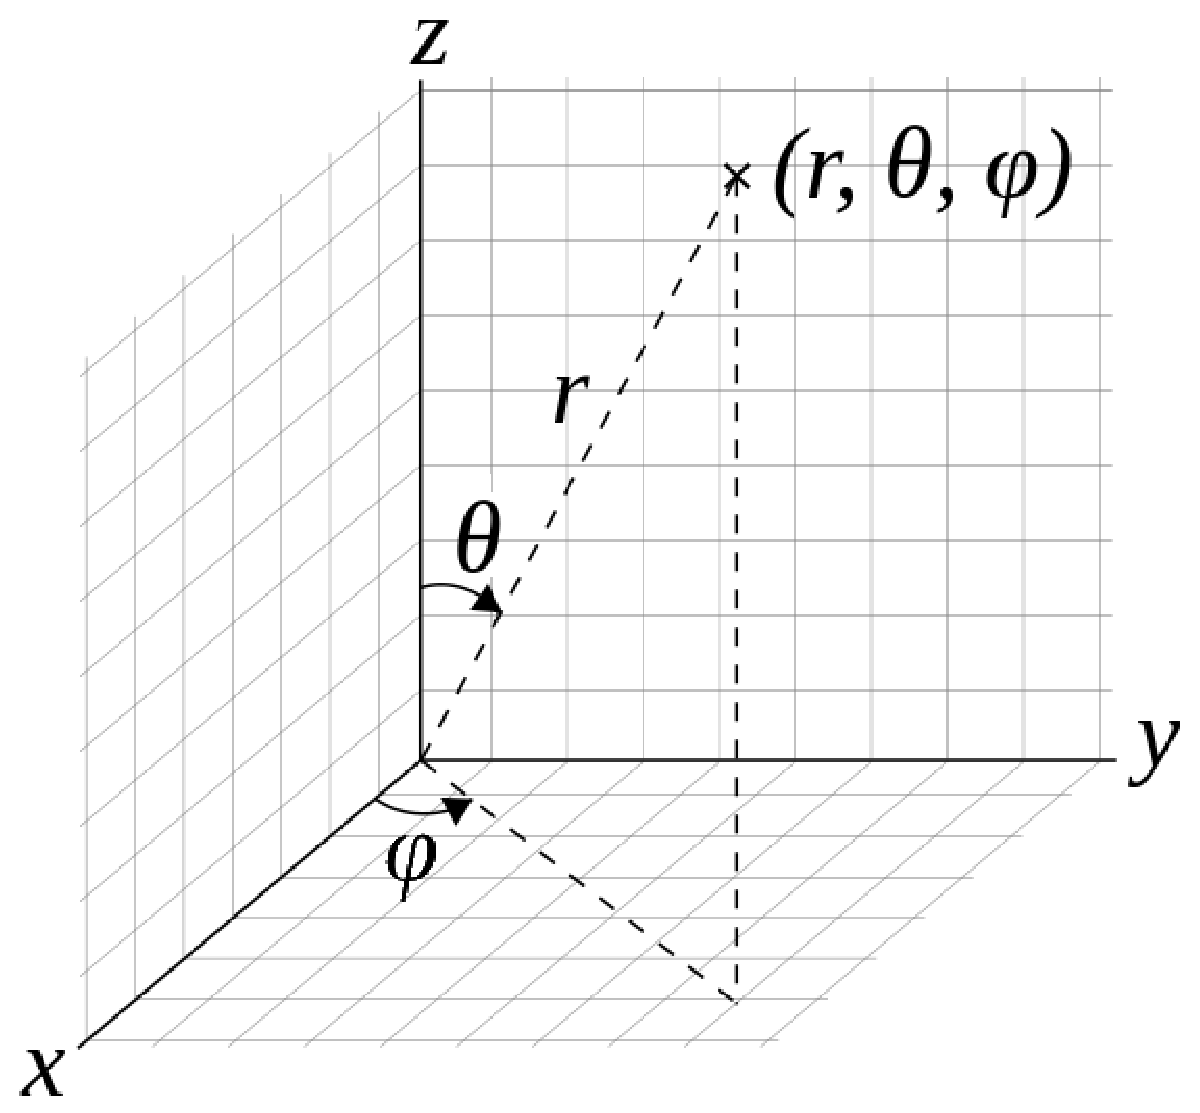
\includegraphics[height=9.5cm]{figure/spheriques_ok.eps}\\
\end{center}

\exo{D\'efinition}
\begin{enumerate}[\bf 1)]
\item   Rappelez l'expression du recouvrement $S_{ab}$, entre une orbitale $ \chi_a(x,y,z)$, et
$\chi_b(x,y,z)$.
\item  Que vaut exactement cette int\'egrale si $ \chi_a(x,y,z)=\chi_b(x,y,z)=\chi(x,y,z)$.
\item    Montrez graphiquement que les orbitales $2s_A$ et $2p_{z_{A}}$ (centr\'ee sur le m\^eme atome A), ont un recouvrement nul. Expliquez.
%\item    A quoi correspond la combinaison  $2s_A+2p_{z_{A}}$~? 
\end{enumerate} %\exo{Variation du Recouvrement avec la distance}
\exo{Recouvrement d'orbitales atomiques}
\label{exo_s}
Dans une mol\'ecule A$-$B, on \'etudie le recouvrement entre 2 orbitales atomiques, l'une centr\'ee sur un atome A, l'autre sur  B. Pour l'ensemble de cet exercice, les axes sont d\'efinis selon la figure du rep\`ere ci-dessous (l'axe internucl\'eaire d\'efinit l'axe Oz, et $x$ est dans le plan de la feuille, vers le haut). 
\\

Pour chaque cas propos\'e,

\begin{minipage}[c]{0.8\linewidth}
\begin{enumerate}[(i)] 
\item dessinez les orbitales en pr\'esence
\item indiquez la nature du recouvrement : $\sigma$, $\pi$ ou nul 
\item  pr\'ecisez s'il s'agit d'un recouvrement positif, n\'egatif ou nul
\end{enumerate} 
\end{minipage}
\begin{minipage}[l]{0.1\linewidth}     
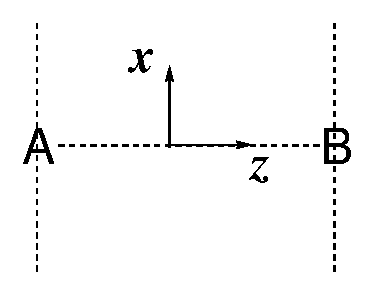
\includegraphics[scale=0.4]{figure/AB_repere.eps}\\   
Rep\`ere
\end{minipage}

\vspace{0.3cm}

\begin{minipage}[c]{0.5\linewidth}
\begin{enumerate}[\bf 1)]
\item $+2p_{x\textsc{a}}\ \, |+\,2p_{x\textsc{b}}$ 
\item $+2p_{z\textsc{a}}\ \, |-\,2p_{z\textsc{b}}$ 
\item $\ \, +2s_\textsc{a}\ \, |+\,2s_\textsc{b}$ 
\item $\ \, +2s_\textsc{a}\ \, |+\,2p_{z\textsc{b}}$ 
\item $+2p_{x\textsc{a}}\ \, |+\,2s_\textsc{b}$ 
%\item $+3p_{y\textsc{a}}\ \, |-\,3p_{y\textsc{b}}$
%\item $-3p_{x\textsc{a}}\ \, |-\,3s_\textsc{b}$
%\item $-2p_{x\textsc{a}}\ \, |-\,3p_{x\textsc{b}}$
\end{enumerate} 
\end{minipage} \hfill
\begin{minipage}[c]{0.5\linewidth}
 \textbf{Exemple :}  $+2s_\textsc{a}\ |-\,2s_\textsc{b}$
\begin{enumerate}[~~(i)] 
\item    Dessin~:\\[-0.3cm] 

   \  \  \  \  \   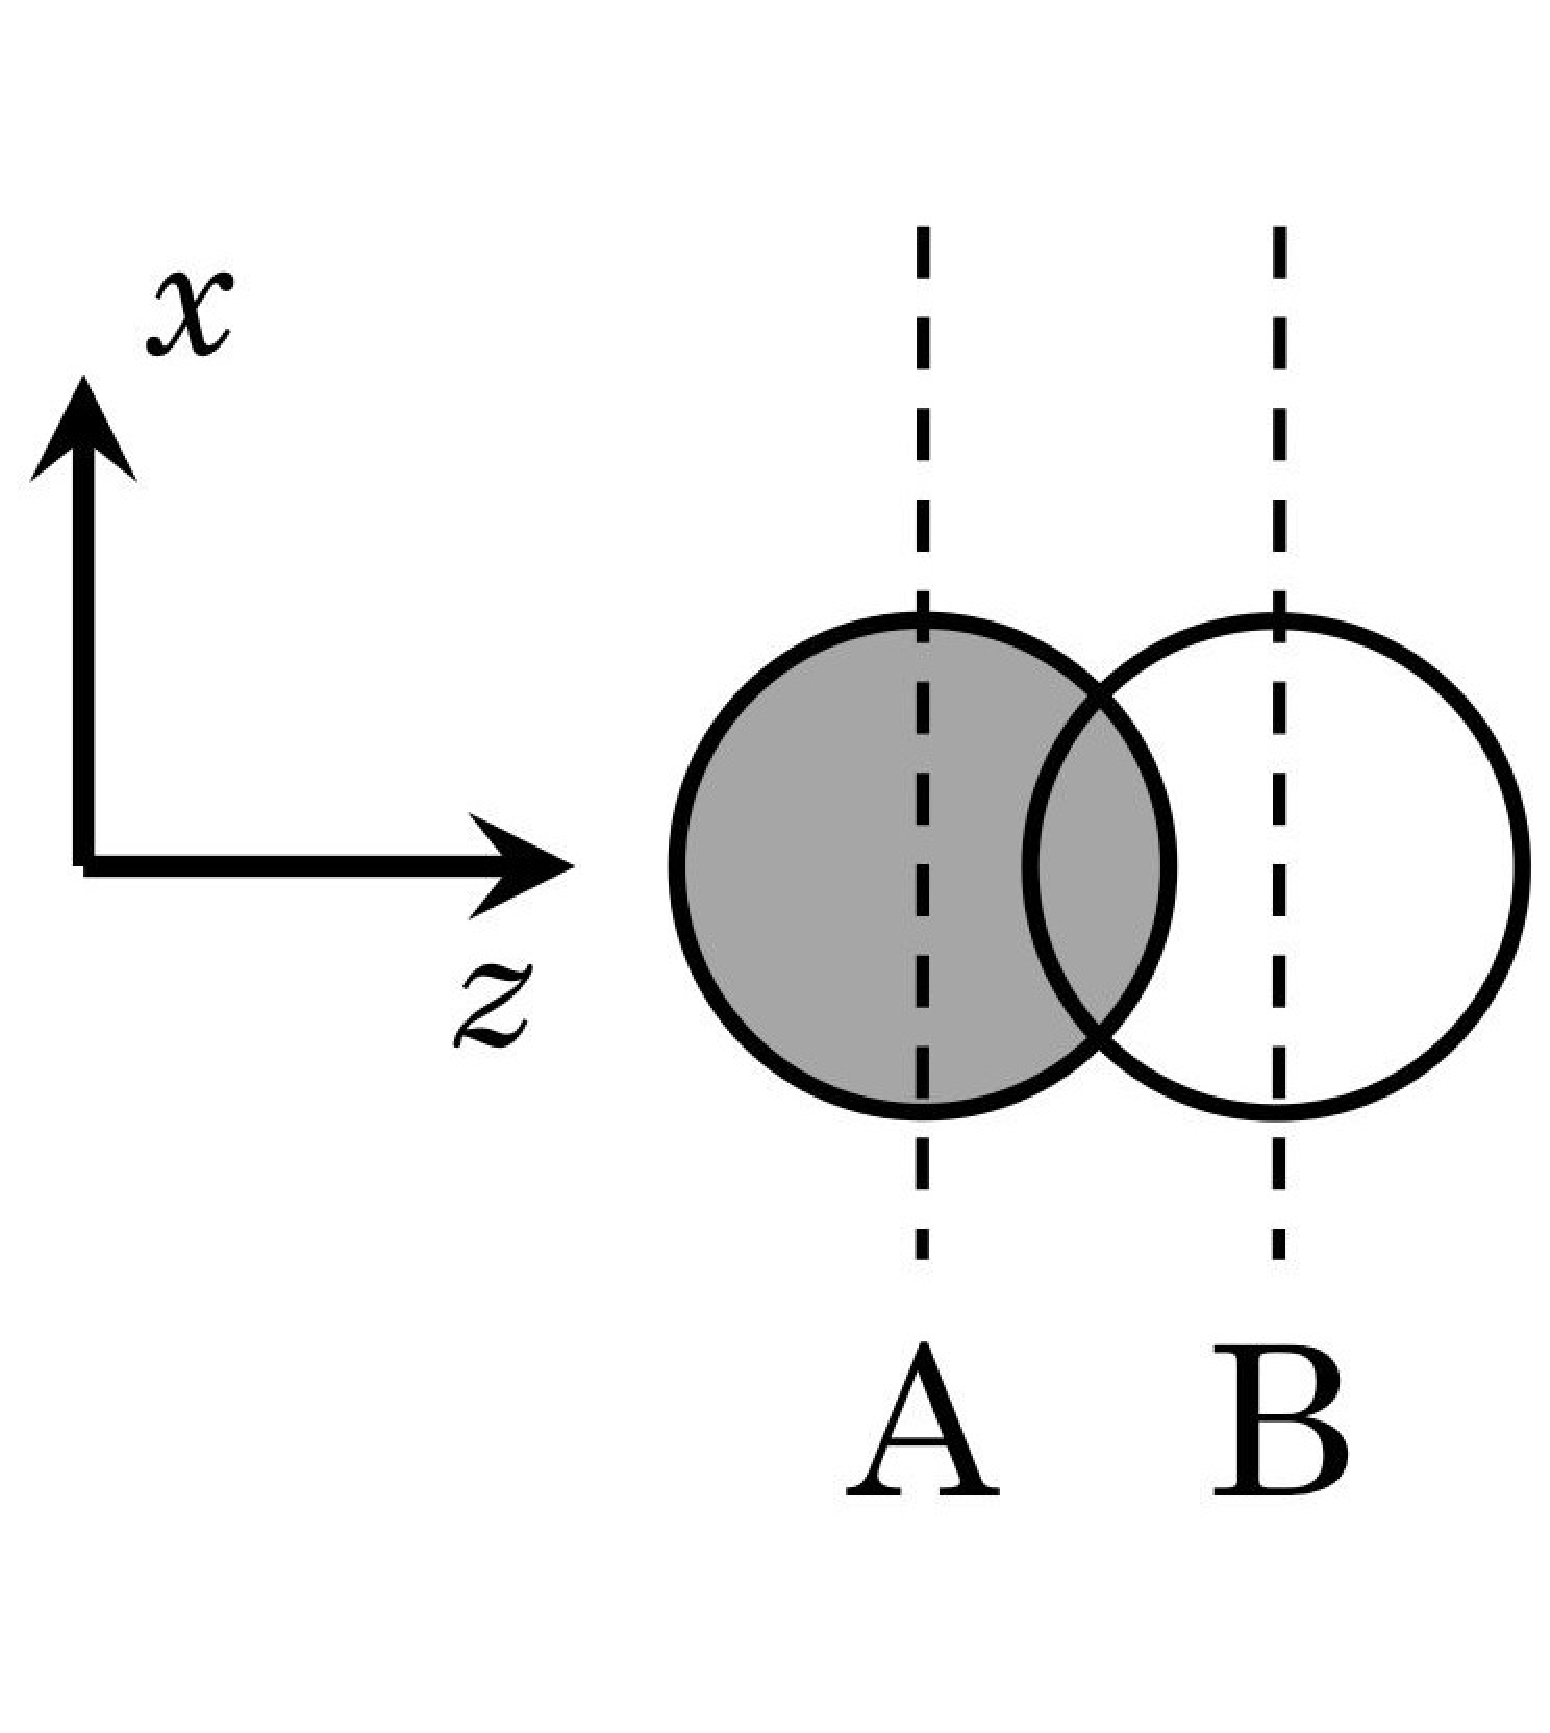
\includegraphics[scale=0.09]{figure/interactionOA.eps}
\item       Recouvrement axial, donc $\sigma$
\item       Recouvrement <0 car de phase $\neq $
\end{enumerate} 
\end{minipage}

%--------------------------------------------------------------------------
\meth{Évolution du recouvrement en fonction de la distance entre deux orbitales}
On consid\`ere une orbitale p$_z$ et une orbitale s qui s'approchent l'une de l'autre.
Dessiner l'allure de l'\'evolution du recouvrement entre elles.\\
\textsl{%
Le recouvrement entre deux orbitales $\phi_a$ et $\phi_b$ est donné par la formule~:
\begin{align*}
S = \int \phi_a \phi_b^* dV
\end{align*}
On peut voir cette intégrale comme une somme sur tout l'espace d'éléments infiniments
petits constitués du produit de ces deux orbitales.
Dans une zone de l'espace où les deux orbitales sont du même signe (même couleur)
le produit est positif.
À l'inverse, si les deux orbitales sont de signes (couleurs) opposés le produit est négatif.
Si la zone où le produit est positif est plus grande que celle où le produit est négatif,
le recouvrement est positif.
Dans les cas où ces deux zones ont exactement la même taille, le recouvrement est nul.
Sinon, il est négatif.
%
De manière à avoir une idée de la forme de la courbe qui donne le recouvrement en fonction
de la distance entre les orbitales, nous allons considérer plusieurs situations dans le tableau suivant~:\\
\hspace*{-8mm}\rotatebox{90}{%
\begin{tabular}{|p{2cm}|p{4cm}|p{7cm}|p{3cm}|}\hline
Distance & Schema & Commentaire & Recouvrement\\\hline
$+\infty$                        & \raisebox{-1cm}{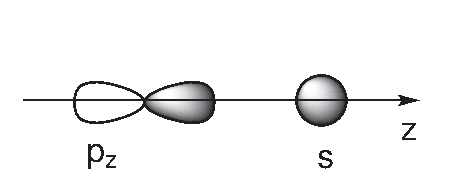
\includegraphics[width=4cm]{figure/ovl01.eps}} & Les orbitales sont sans interaction. & nul \\\hline
positive et grande               & \raisebox{-1cm}{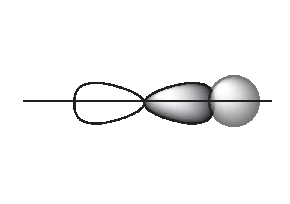
\includegraphics[width=3cm]{figure/ovl02.eps}} & Les orbitales interagissent faiblement. Dans cette zone elles sont toutes les deux du même signe (colorées). & petite valeur positive \\\hline
proche de la distance de liaison & \raisebox{-1cm}{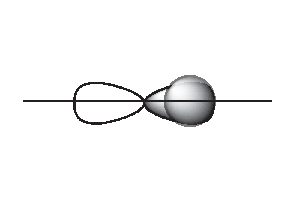
\includegraphics[width=3cm]{figure/ovl03.eps}} & Les orbitales se recouvrent largement: le recouvrement atteint sa valeur maximale.                           & positif et maximum    \\\hline
positive et courte               & \raisebox{-1cm}{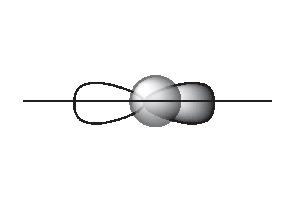
\includegraphics[width=3cm]{figure/ovl04.eps}} & Une partie des orbitales se recouvre avec un signe opposé (blanc et coloré) ce qui diminue le recouvrement.& petite valeur positive \\\hline
nulle                            & \raisebox{-1cm}{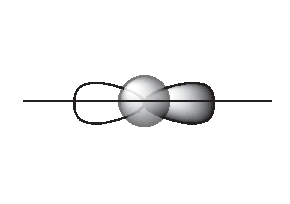
\includegraphics[width=3cm]{figure/ovl05.eps}} & La partie positive du recouvrement (lorsque les orbitales sont du même signe) est égale en valeur absolue à sa partie négative. & nul \\\hline
négative et courte               & \raisebox{-1cm}{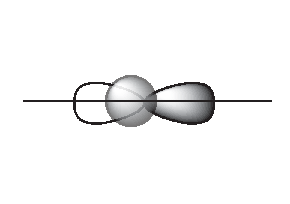
\includegraphics[width=3cm]{figure/ovl06.eps}} & Une partie des orbitales se recouvre avec un même signe ce qui diminue la valeur absolu du recouvrement.& petite valeur négative \\\hline
\end{tabular}
}\\
On obtient alors le graphe suivant~:\\
\begin{center}
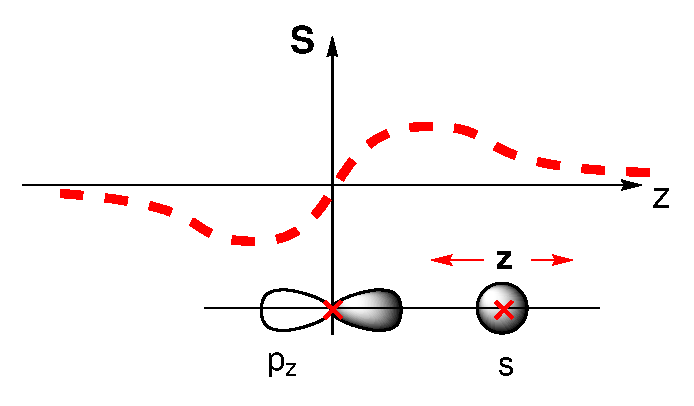
\includegraphics[width=8.0cm]{figure/exempl_recou_zs.eps}
\end{center}
}

\exo{Recouvrement entre orbitales}

Les dessins des orbitales donnent la forme g\'en\'erale du volume o\`u l'\'electron
a le plus de chance de se trouver. M\^eme quand ces orbitales ne se touchent pas
graphiquement, on a un recouvrement.

On consid\`ere deux orbitales qui s'approchent l'une de l'autre.
Dessiner l'allure de l'\'evolution du recouvrement entre les diff\'erentes orbitales
pour $z \in ]-\infty;+\infty[$.

%%FIGURE
\vspace{-0.3cm}
\begin{center}
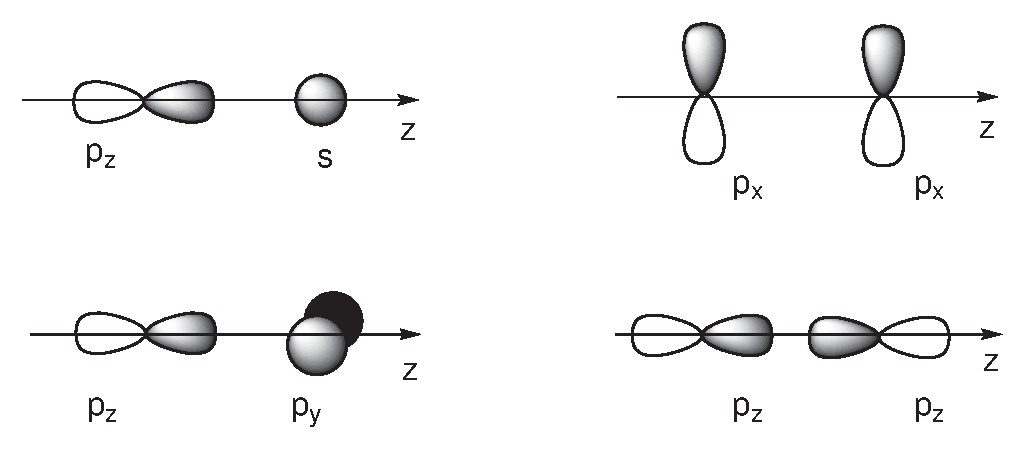
\includegraphics[width=8.0cm]{figure/overl1.eps}
\end{center}

\exo{Matrice de recouvrement}

Dans cet exercice le rep\`ere est defini de la mani\`ere suivante~:

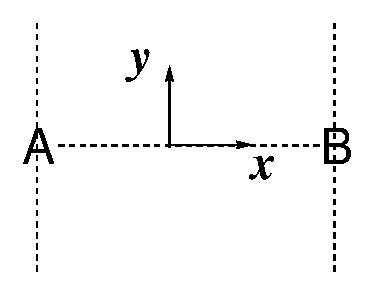
\includegraphics[width=2cm]{figure/AB_repere_yx.eps}

Pour deux atomes, A et B, s\'epar\'es d'une distance de liaison 
(environ 1.0-2.0~\AA), remplissez le tableau suivant avec les valeurs 0, 1 et $+$ ou $-$
selon la signe du recouvrement~:
%\begin{enumerate}
%\item $\chi_i = 1s_\textsc{a}$ et $\chi_j = 1s_\textsc{b}$~;
%\item $\chi_i = 2s_\textsc{a}$ et $\chi_j = 2s_\textsc{b}$~;
%\item $\chi_i = 2s_\textsc{a}$ et $\chi_j = 2p_{x\textsc{b}}$~;
%\end{enumerate}
%
%\item Remplissez le tableau suivant~:

\begin{tabular}{|c||c|c|c|c|c|}
\hline
                   & $2s_\textsc{a}$ & $2s_\textsc{b}$ & $2p_{x\textsc{b}}$ & $2p_{y\textsc{b}}$ & $2p_{z\textsc{b}}$ \\
\hline\hline
$2s_\textsc{a}$     & 1 & $+$ & $-$ & 0 & 0 \\ \hline
$2s_\textsc{b}$     &&&&& \\ \hline
$2p_{x\textsc{b}}$  &&&&& \\ \hline
$2p_{y\textsc{b}}$  &&&&& \\ \hline
$2p_{z\textsc{b}}$  &&&&& \\ \hline
\end{tabular}
